\documentclass[12pt]{article}

\usepackage[margin=1.0in]{geometry}
\usepackage{graphicx}
\usepackage{listings}
\usepackage{tabto}
\usepackage{multicol}
\usepackage{lipsum}
\usepackage{caption}
\usepackage{mwe}
\usepackage{tikz}
\usepackage{tabto}
\usetikzlibrary{automata,positioning}
\usepackage{enumitem}
\usepackage{amsmath}
\usepackage{amssymb}
\graphicspath{ {./} }

\usepackage{graphicx}
\usepackage[colorlinks=true, pdfstartview=FitV, linkcolor=blue, citecolor=blue, urlcolor=blue]{hyperref}
\usepackage[hyphenbreaks]{breakurl}
\usepackage[space]{grffile}% used to allow spaces within the filenames
\newread\reader
\newcommand\IterateLines[2]{
    \immediate\write18{ls -1 "#1" > \jobname.txt}
    \openin\reader=\jobname.txt\relax
    \endlinechar=-1
    \loop
    \read\reader to \line
    \unless\ifeof\reader
    {\line}\par
    \includegraphics[width=2cm]{{#1\line}} %
    \par
    \repeat
    \closein\reader
}
\makeatother


\lstset{language=sql,%
    %basicstyle=\color{red},
    breaklines=true,%
    morekeywords={matlab2tikz},
    morekeywords=[2]{1}, keywordstyle=[2]{\color{black}},
    identifierstyle=\color{black},%
    showstringspaces=false,%without this there will be a symbol in the places where there is a space
    numbers=left,%
    numberstyle={\tiny \color{black}},% size of the numbers
    numbersep=9pt, % this defines how far the numbers are from the text
    emph=[1]{for,end,break},emphstyle=[1]\color{red}, %some words to emphasise
    %emph=[2]{word1,word2}, emphstyle=[2]{style},    
}


\begin{document}

\title{CS4337 : Database Systems\\Term Project Write-up}
\author{Matthew McMillian\\mgm160130@utdallas.edu}
\maketitle


\begin{enumerate}
	
	\item Problem Description:	
	\begin{center}
		Our objective in this project is to design and implement a database based on the given criteria. Our database resembles that of a business, containing tables relating to employees, customers, products, etc. Using the information given, we are tasked with designing multiple distinct diagrams such as a Relational, Conceptual EER, and Logical EER diagram. Then, we are tasked with defining views to display a subset of our data and we are supposed to implement queries for data retrieval.
	\end{center}
	
	\item Project Questions:
		\begin{enumerate}
			\item Can you think of 5 more rules (other than the ones explicitly described above) that are likely to be used in a company? \\
				\begin{itemize}
					\item Departments would have teams of employees. In leu of this, employees would also belong to teams.
					\item  As well as marketing sites, there could be offices that different (and sometimes the same departments) and employees would work at, and it might be useful to keep track of this information.
					\item As we've seen in the textbook, for insurance reasons it may be beneficial to keep track of employees dependents.
					\item As we've seen in the textbook, teams or groups of employees have projects to work on. Adding a project entity to keep track of the work done by employees would be beneficial.
					\item If we have projects, we would need a relation for a department to control a project (since it has to be assigned somewhere).
				\end{itemize}
				
		\pagebreak
				
			\item Is the ability to model super-class/subclass relationships likely to be important in such an environment? Why or why not?
			\begin{itemize}
			\item It is important to model this superclass / subclass relationship. In this environment, we have many different types of people
      that we can interact with at the company. These people also have differing attributes to them. For example, we would not want
      a customer to have a salary. More generally, we don't want or care to keep track of a customers information such as their name,
      sex, birth date, ... since it would be useless information. Having the ability to categorize these types of potential people
      can make it easy to store data efficiently and not overpopulate tables.
			\end{itemize}
			
			\item Justify using a Relational DBMS like Oracle for this project.
				\begin{itemize}
					 \item In a company it is important to have consistent information. Especially in an enterprise environment, data is flowing in and out
      at rapid speeds. Because of this we need a database structure that supports atomic operations (CRUD operations) so that we can
      preserve the integrity of our fast-paced data. Another thing that a company structure has is a variety of data. Since almost all
      the entities in our database are related in some way, it may be useful to perform joins to get specific subsets of data. In a
      Non-Relational DBMS joins are nonexistent. To even simulate what a join can do, you would have to perform multiple queries which
      can be very inefficient. Due to our atomicity and relational constraints listed above, it is safe to say that in this scenario a
      Relational DBMS can be used to store our data.
				\end{itemize}			
		\end{enumerate}
		
		\pagebreak
		
		\item Project Diagrams: 
			\begin{itemize}
				\item Relational Diagram: (Note this is in 3NF)
				\begin{center}
					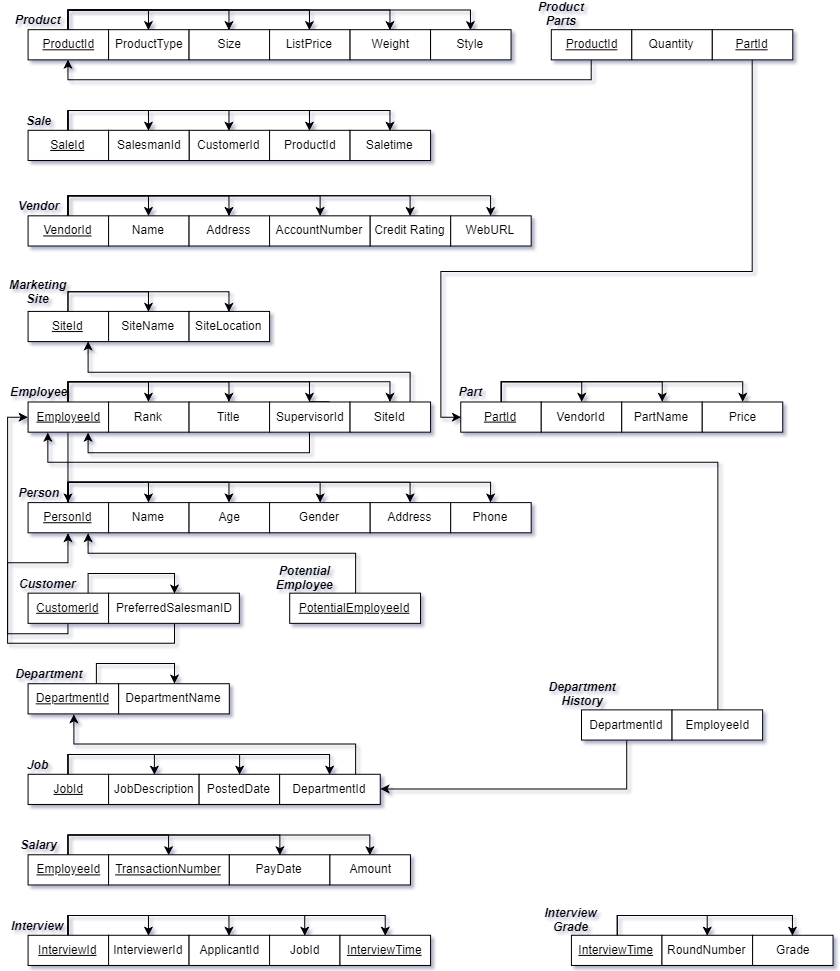
\includegraphics[scale=.5]{completed_diags/conceptual}
				\end{center}
				
				\pagebreak
				
				\item EER Diagram:
				\begin{center}
					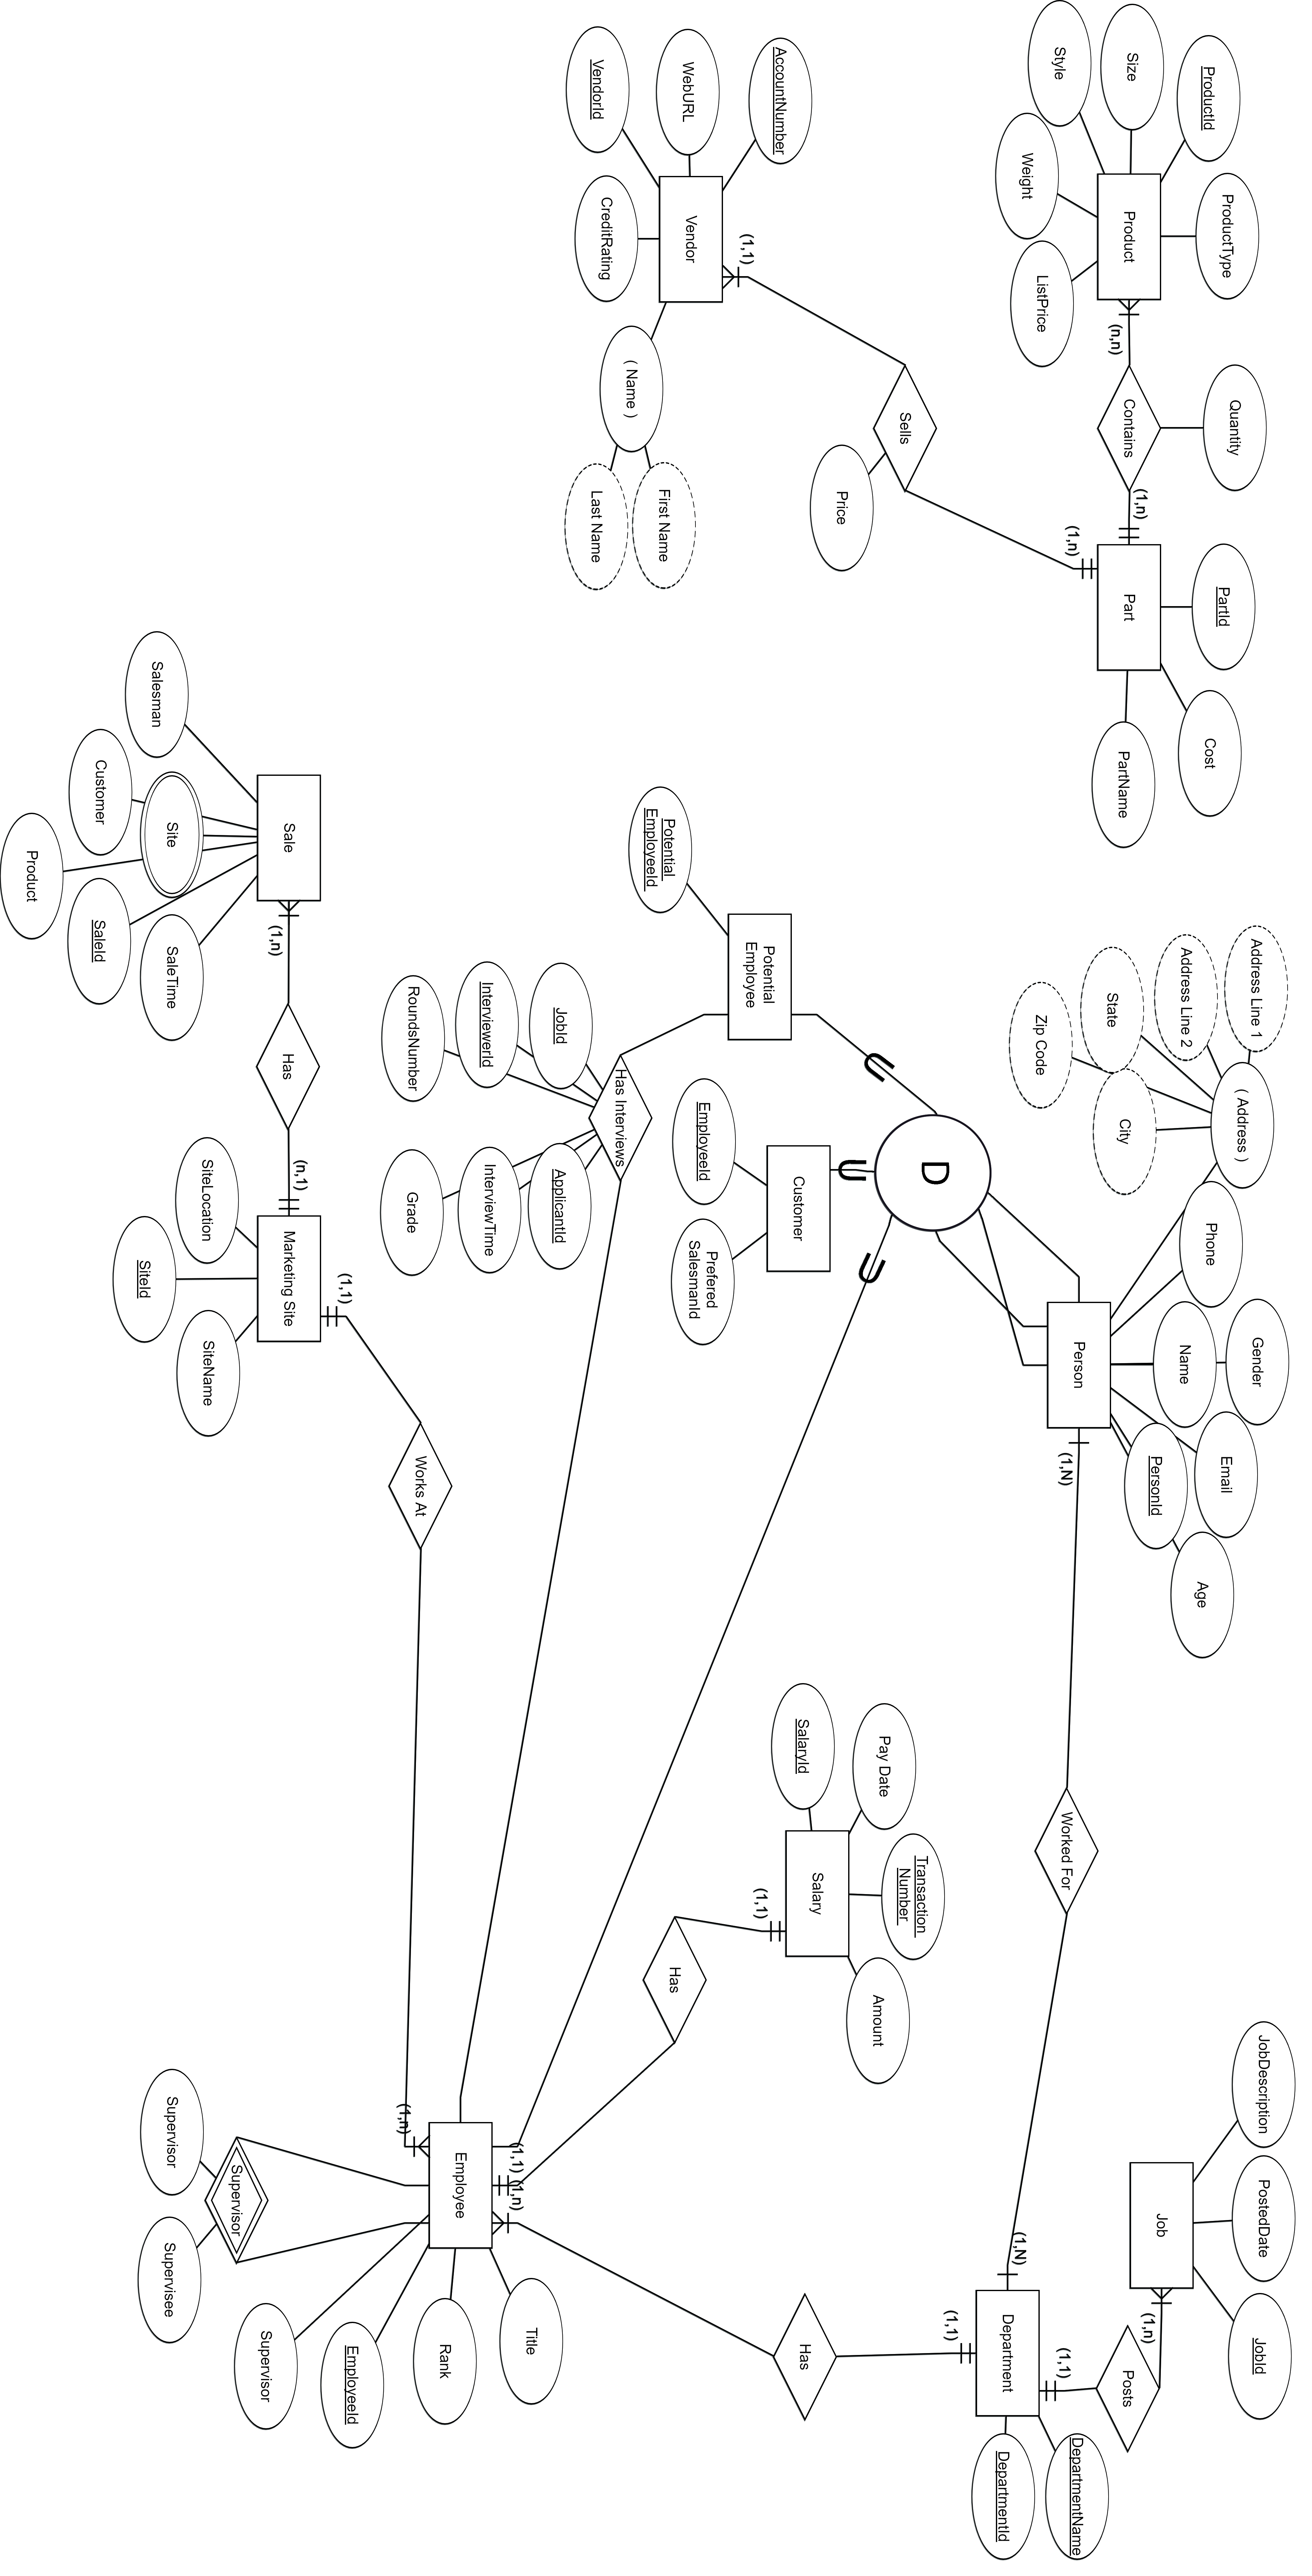
\includegraphics[scale=.075]{completed_diags/eer_rot}
				\end{center}
			
			\end{itemize}

		\pagebreak			
			
		\item SQL Statements
			\begin{itemize}
				\item \textbf{Database Views:}
				\lstinputlisting{DBViews.sql}		
				
				\pagebreak

				\item \textbf{Database Creation:}
				\lstinputlisting{DBCreation.sql}
				
				\pagebreak				
				
				\item \textbf{Database Insertion (For Testing):}
				\lstinputlisting{DBInsert.sql}						
				
				\pagebreak				
				
				\item \textbf{Database Queries:}
				\lstinputlisting{DBQueries.sql}	
			\end{itemize}
	
		\item Dependency Diagram:
			\begin{center}
				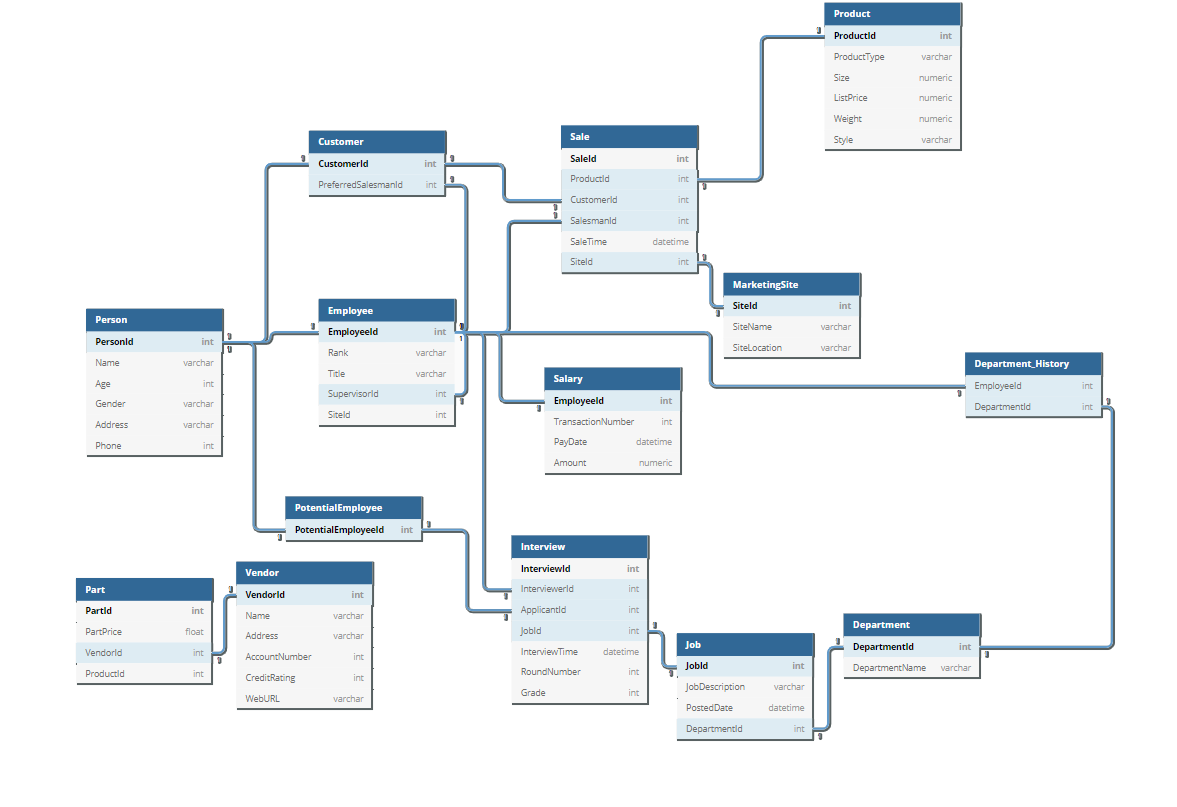
\includegraphics[scale=.55]{completed_diags/depend}
			\end{center}
		
		\item Database States:
		\begin{center}
				Customer:\\
				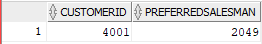
\includegraphics[scale=1.5]{completed_diags/states/customer}
		\end{center}
		\begin{center}
				Department:\\
				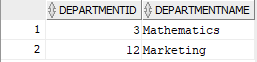
\includegraphics[scale=1.5]{completed_diags/states/department}
		\end{center}
		\begin{center}
				Department History:\\
				\includegraphics[scale=1.5]{completed_diags/states/department_history}
		\end{center}
		\begin{center}
				Employee:\\
				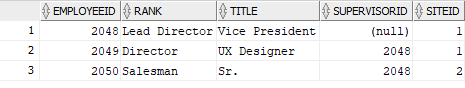
\includegraphics[scale=1.2]{completed_diags/states/Employee}
		\end{center}
		\begin{center}
				Interview:\\
				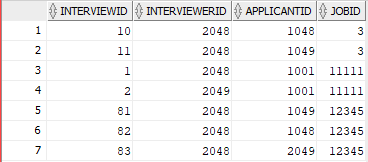
\includegraphics[scale=1.5]{completed_diags/states/interview}
		\end{center}
		\begin{center}
				Interview Grade:\\
				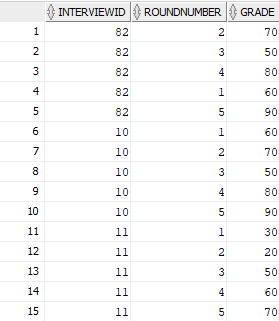
\includegraphics[scale=1.5]{completed_diags/states/Interview_grade}
		\end{center}
		\begin{center}
				Job:\\
				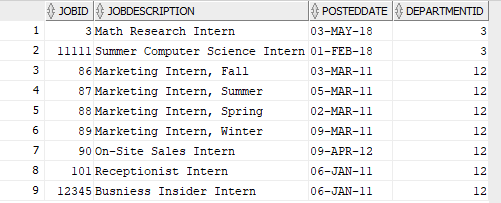
\includegraphics[scale=1.0]{completed_diags/states/Job}
		\end{center}
		\begin{center}
				MarketingSite:\\
				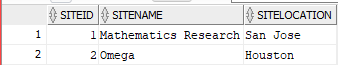
\includegraphics[scale=1.5]{completed_diags/states/MarketingSite}
		\end{center}
		\begin{center}
				Part:\\
				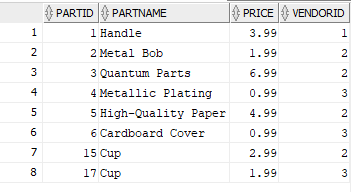
\includegraphics[scale=1.5]{completed_diags/states/Part}
		\end{center}
		\begin{center}
				Person:\\
				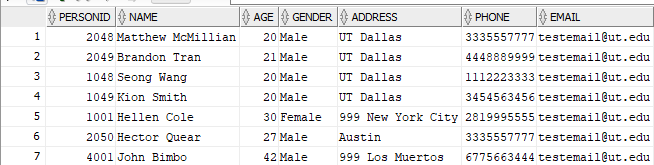
\includegraphics[scale=1.0]{completed_diags/states/person}
		\end{center}
		\begin{center}
				Potential Employee:\\
				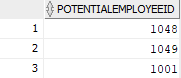
\includegraphics[scale=1.5]{completed_diags/states/PotentialEmployee}
		\end{center}
		\begin{center}
				Product:\\
				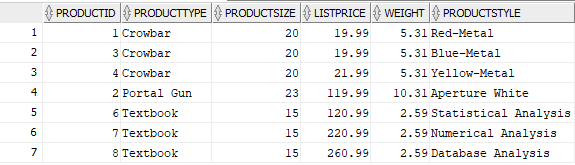
\includegraphics[scale=1.0]{completed_diags/states/Product}
		\end{center}
		\begin{center}
				Product Parts:\\
				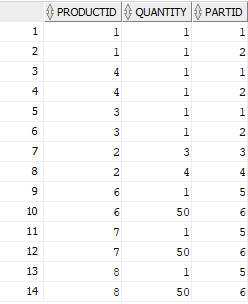
\includegraphics[scale=1.5]{completed_diags/states/Product_Parts}
		\end{center}
		\begin{center}
				Salary:\\
				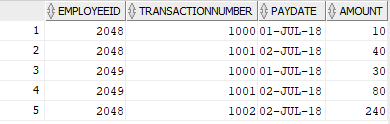
\includegraphics[scale=1.5]{completed_diags/states/Salary}
		\end{center}
		\begin{center}
				Sale:\\
				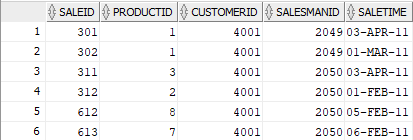
\includegraphics[scale=1.5]{completed_diags/states/Sale}
		\end{center}
		\begin{center}
				Vendor:\\
				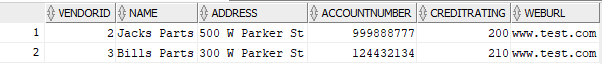
\includegraphics[scale=1.0]{completed_diags/states/vendor}
		\end{center}
		\begin{center}
				View 1:\\
				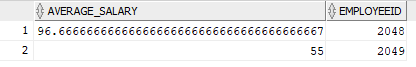
\includegraphics[scale=1.0]{completed_diags/states/view1}
		\end{center}
		\begin{center}
				View 2:\\
				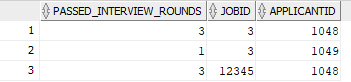
\includegraphics[scale=1.0]{completed_diags/states/view2}
		\end{center}
		\begin{center}
				View 3:\\
				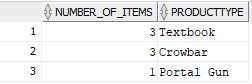
\includegraphics[scale=1.0]{completed_diags/states/view3}
		\end{center}		
		\begin{center}
				View 4:\\
				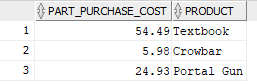
\includegraphics[scale=1.0]{completed_diags/states/view4}
		\end{center}	
\end{enumerate}


\end{document}
